\documentclass[12pt,twoside]{article}
\usepackage{jmlda}
\newcommand{\hdir}{.}
\usepackage{hyperref}       % clickable links
\usepackage{lineno}
\usepackage{graphicx,multicol}
\usepackage{cite}
\usepackage{tikz}
\usetikzlibrary{shapes,arrows,shadows}
\newtheorem{theorem}{Теорема}

\bibliographystyle{jmlda_eng}
%\renewcommand{\baselinestretch}{1.4}


\newcommand{\bx}{\mathbf{x}}
\newcommand{\by}{\mathbf{y}}
\newcommand{\bw}{\mathbf{w}}
\newcommand{\bY}{\mathbf{Y}}
\newcommand{\bX}{\mathbf{X}}
\newcommand{\bu}{\mathbf{u}}
\newcommand{\bt}{\mathbf{t}}
\newcommand{\bp}{\mathbf{p}}
\newcommand{\bq}{\mathbf{q}}
\newcommand{\bg}{\mathbf{g}}
\newcommand{\bh}{\mathbf{h}}
\newcommand{\bv}{\mathbf{v}}
\newcommand{\be}{\mathbf{e}}
\newcommand{\bc}{\mathbf{c}}
\newcommand{\bP}{\mathbf{P}}
\newcommand{\bT}{\mathbf{T}}
\newcommand{\bQ}{\mathbf{Q}}
\newcommand{\bC}{\mathbf{C}}
\newcommand{\bE}{\mathbf{E}}
\newcommand{\bF}{\mathbf{F}}
\newcommand{\bU}{\mathbf{U}}
\newcommand{\bW}{\mathbf{W}}
\newcommand{\bD}{\mathbf{D}}
\newcommand{\bI}{\mathbf{I}}
\newcommand{\bJ}{\mathbf{J}}
\newcommand{\bB}{\mathbf{B}}
\newcommand{\btheta}{\boldsymbol{\theta}}
\newcommand{\bTheta}{\boldsymbol{\Theta}}



\title
	{Нелинейное снижение размерности в задачах декодирования временных рядов и прогнозирования}
\author
	{Мария Владимирова, Роман Исаченко}
\email
    {\href{mailto:vladimirova.maria@phystech.edu}{vladimirova.maria@phystech.edu}, 
    \href{mailto:isa-ro@yandex.ru}{isa-ro@yandex.ru}}
\organization
    {Московский физико-технический институт}
\abstract
	{В работе решается задача обнаружения зависимостей в прогнозируемой переменной. 
    Используется набор гомогенных моделей, восстанавливающих прогноз по общему для всех переменных описанию объектов. 
    Рассматривается линейная модель метода частный наименьших квадратов и ее предложенная нелинейная модификация. 
    Находятся оптимальные параметрические преобразования исходных пространств объектов и ответов. 
    Проводится вычислительный эксперимент на реальных данных объемов потребления электроэнергии и данных сигналов кортикограмм.

    \bigskip
	\noindent
	\textbf{Ключевые слова}: \emph {прогнозирование временных рядов; мультиколлинеарность; метод частных наименьших квадратов; PLS; нелинейный PLS} 
	}

\thanks{Проект поддержан грантом РФФИ \No 16-07-01155.}


\begin{document}
\maketitle


\linenumbers
%%%%%%%%%%%%%%%%%%%%%%%%%%%%%%%%%%%%%%%%%%%%%%%%%%%%%%%%%%%%%%%%%%%%%%%%%%%%%%
\section{1. Введение}
%%%%%%%%%%%%%%%%%%%%%%%%%%%%%%%%%%%%%%%%%%%%%%%%%%%%%%%%%%%%%%%%%%%%%%%%%%%%%%
В работе рассматривается задача прогнозирования временных рядов в случае наличия мультиколлинеарности в данных. Методы решения данной задачи сравниваются на двух наборах данных, имеющих избыточную информацию. 

Первый набор данных представляет собой временные ряды объема потребления электроэнергии в Варшаве. 
% Также в работе рассматривается задача прогнозирования потребления электроэнегрии на основе исторических данных. 
Электрическая энергия является важной движущей силой экономического развития, а точность прогнозов спроса является важным фактором, который ведет к успешному эффективному планированию. 
По этой причине энергетическим аналитикам необходимо руководство для лучшего выбора наиболее подходящих методов прогнозирования, чтобы обеспечить точные прогнозы тенденций потребления электроэнергии.
Предполагается, что значение сигнала в данный момент времени линейно зависит от предыдущих значений этого же сигнала, поэтому данные являются мультиколлинеарными.  


Второй набор данных взят из проекта Project Tycho, в котором изучалась проблема проектирования нейро-компьютерного интерфейса (BCI) для обмена информацией между мозгом и электронным устройством. Решается задача выбора функций в моделях регрессии в приложении к декодированию движения на основе электрокардиограмм (ECoG). 
Проблема состоит в том, чтобы предсказать траектории руки из временных рядов напряжения кортикальной активности. Описание функции каждой точки находится в пространственно-временной частотной области включает в себя сами временные ряды напряжения и их спектральные характеристики. Выбор функции имеет решающее значение для адекватного решения проблемы регрессии, поскольку электрокортикальные данные являются высокомерными и измерения коррелируют как во временной, так и в пространственной областях.

Система BCI улучшает умственные и физические возможности пользователя, обеспечивая прямую связь между мозгом и компьютером. BCI направлены на восстановление поврежденных функциональных возможностей пациентов с механическими или когнитивными нарушениями. В данной статье предлагается новый метод выбора признаков в прогнозировании движения и его реконструкции.
% Анализ кортикальной активности во время моторных изображений необходим для проектирования BCI. Цель анализа автомобильных изображений заключается в распознавании предполагаемых движений из зарегистрированной активности мозга. Хотя существуют различные методы измерения кортикальных данных для BCI \textcolor{red}{ссылки},
% % [14, 1]
% , мы концентрируемся на сигналах ElectroCorticoGraphic (ECoG) [10]. ECoG, а также другие инвазивные методы обеспечивают более стабильные записи и лучшее разрешение во временных и пространственных областях, чем его неинвазивные аналоги.
Первый шагом к прогнозированию предполагаемых движений~---~научиться реконструировать фактические перемещения из кортикальной активности. Рассматривается проблема непрерывной реконструкции траектории. Субдуральные сигналы ECoG измеряются через 32 или 64 канала, когда субъект перемещает руку. 
% \textcolor{red}{ссылки}. 
% [18]. 
Когда сигналы ECoG трансформируются в информационные функции, проблема восстановления траектории является проблемой регрессии. Извлечение функции включает в себя применение некоторого спектрально-временного преобразования к сигналам ECoG с каждого канала. 
% \textcolor{red}{ссылки}.
% [13, 15, 9]. 
Так как результирующее пространственно-временное спектральное представление сильно избыточно, используются различные методы выбора объектов и уменьшения размерности,  
% \textcolor{red}{ссылки}, 
% [17, 16]
чтобы извлечь только наиболее важные функции.
% Многостороннее представление активно используется при анализе биоматериалов и химических данных благодаря многоходовой структуре данных в этих областях. Развертывание многоходовых данных в плоские матрицы может привести к пренебрежению важными зависимостями, присутствующими в развернутом измерении многопоточных данных. Напротив, многосторонние подходы сохраняют структуру данных и улучшают качество регрессии, что было продемонстрировано в \textcolor{red}{ссылка}
% % [17] 
% для регрессии частичных наименьших квадратов (PLS). Регрессия PLS и ее расширения для многопутевых данных \textcolor{red}{ссылки}
% % [10, 17] 
% доказали свою эффективность в реконструкции траектории ручной работы на ECoG \textcolor{red}{ссылки}.
% [17, 9, 7]
% Аналогично оригинальной PLS, основанной на разложении сингулярных значений, многопоточные расширения PLS полагаются на многопоточные разложения, такие как разложение Tucker или PARAFAC \textcolor{red}{ссылка}
% % [8]. 
% Кроме того, было предложено несколько методов регуляризации для повышения его стабильности \textcolor{red}{ссылка}
% % [10] 
% и сокращения переобучения.


Для решения задачи прогнозирования используется авторегрессионная модель. 
Авторегрессионная модель является неустойчивой в случае наличия мультиколлинеарности в исторических данных. 
Для решения этой проблемы необходимо используются методы отбора признаков~\cite{Li2016}, в результате чего повышается устойчивость модели без существенного снижения качества прогноза.

В работе исследуются методы отбора признаков: метод частных наименьших квадратов (PLS) \cite{Ng2013} и предложенная его нелинейная модицикация (cnlPLS).
Метод частных наименьших квадратов основан на снижении размерности матрицы признаков и выделяет линейные комбинации признаков, которые оказывают наибольшее влияние на вектор ответов. 
Выделение признаков происходит итеративно, в порядке уменьшения их влияния на вектор ответов \cite{Ng2013}. Рассматриваются только значимые комбинации признаков, незначительно потеряв в точности прогноза. 

Методы PLS регрессии подробно описаны в работах~\cite{Geladi1988, Hoskuldsson1988}. 
Разницу между методом PLS и связанными с ним подходами, различные разновидности регрессии PLS можно найти в~\cite{Lehky2014}.

Нелинейное расширение метода PLS регрессии впервые введено в~\cite{Frank1990}. 
В литературе были разработаны различные модификации PLS. 
Предложены нелинейные методы PLS, основанные на различных моделях:  искусственных нейронных сетей~\cite{Mcavovt1992}, функции активации радиальных оснований\cite{Yan2003}, логистическая функция активации и методы оптимизации роевых частиц~\cite{Zhou2007}, используют прямые нейронные сети~\cite{Xuefeng2010}, искусственую нейронную сеть Эльмана~\cite{Bulut2014}.

Предлагается провести модификацию алгоритма PLS: совершить криволинейное и нелинейное преобразования пространства целевой переменной для учета зависимостей между сигналами в разные моменты времени.


В работе проведено сравнение двух методов отбора признаков в задаче авторегрессионного прогнозирования сигналов (PLSR и cnlPLSR). 
Цель регрессии PLS~\cite{Abdi2003}~---предсказать $\bY$ по $\bX$ и описать их общую структуру. 
Когда $\bY$~--- вектор, а $\bX$~--- матрица полного ранга, эта цель может быть выполнена с использованием обычной линейной регрессии. 
Если число предикторов велико по сравнению с числом наблюдений, то $\bX$ будет сингулярной и регрессионный подход в этом случае невозможен из-за наличия мультиколлинеарности.

В качестве практической проверки данных методов в ходе вычислительного эксперимента решается задача прогнозирования на реальных данных.
Результатом применения отбора признаков является снижение размерности задачи и повышение устойчивости моделей без существенной потери точности прогноза.
 
%%%%%%%%%%%%%%%%%%%%%%%%%%%%%%%%%%%%%%%%%%%%%%%%%%%%%%%%%%%%%%%%%%%%%%%%%%%%%%

\section{Постановка задачи}
%%%%%%%%%%%%%%%%%%%%%%%%%%%%%%%%%%%%%%%%%%%%%%%%%%%%%%%%%%%%%%%%%%%%%%%%%%%%%%
Задана выборка $\mathfrak{D}= \left( \bX, \bY \right)$, где $\mathbf{X} \in \mathbb{R}^{m \times n}$~--- матрица объектов, $\mathbf{Y} $~--- матрица ответов. 
Строки матрицы $\bX$ являются объектами из некоторого множества $\mathbb{X} \subset \mathbb{R}^{n}$. Каждому объекту соответствует ответ из некоторого множества $\mathbb{Y} \subset \mathbb{R}^r$.
Способ построения выборки под определенную прикладную задачу описан в разделе "Вычислительный эксперимент".

Предположим, что между объектами $\bx \in \mathbb{X} \subset \mathbb{R}^n$ и ответами $\by \in \mathbb{Y} \subset \mathbb{R}^r$ существует линейная зависимость 
\begin{equation}
\by = \bx \bTheta + \boldsymbol{\epsilon}, 
\label{eq::model}
\end{equation}
где $\bTheta \in \mathbb{R}^{n \times r}$~---~матрица параметров модели, а~$\boldsymbol{\epsilon}\in \mathbb{R}^{r}$~---~вектор регрессионных остатков.

Необходимо по известной выборке $\mathfrak{D}$ восстановить матрицу параметров модели~\eqref{eq::model}.
Оптимальные параметры находятся минимизацией функции ошибки.
Введем квадратичную функцию ошибки $S$ на выборке $\mathfrak{D}$:
\begin{equation}
	S(\bTheta | \mathfrak{D}) = {\bigl\| \mathbf{X}\bTheta - \mathbf{Y} \bigr\| }_2^2 = \sum_{i=1}^m \| \bx_i \bTheta - \by_i\|_2^2 \rightarrow\min_{\bTheta}.
\label{eq::error_function}
\end{equation}
 
Линейная зависимость столбцов матрицы $\bX$ приводит к неустойчивому решению задачи оптимизации~\eqref{eq::error_function}. Для устранения линейной зависимости применяются методы отбора признаков.

\section{Метод частных наименьших квадратов (PLS)}

Для устранения линейной зависимости и снижения размерности пространства применяется метод главных компонент. 
Основным недостатком данного метода является то, что он не учитывает взаимосвязь между объектами и ответами.
Метод частных наименьших квадратов проецирует пространство объектов $\mathbb{X}$ и пространство ответов $\mathbb{Y}$ в латентное пространство $\mathbb{Z}$ меньшей размерности. В отличие от метода главных компонент, метод частных наименьших квадратов учитывает взаимосвязь между матрицами $\bX$ и $\bY$ и снижает размерность  пространства объектов.

Матрица плана $\bX$ и матрица ответов $\bY$ проецируются на пространство $\mathbb{Z}$ размерности~$l$ ($l < n$) следующим образом:

\begin{align}
\label{pls_x_y}
 \underset{m \times n}{\vphantom{\bQ}\bX} &= \underset{m \times l}{\vphantom{\bQ}\bT} \cdot \underset{l \times n}{\vphantom{\bQ}\bP^{\T}} + \underset{m \times n}{\vphantom{\bQ}\bE},\\
 \underset{m \times r}{\vphantom{\bQ}\bY} &= \underset{m \times l}{\vphantom{\bQ}\bU} \cdot \underset{l \times r}{\bQ^{\T}} + \underset{m \times r}{\vphantom{\bQ}\bF},
\end{align}
где $\bT,\ \bU$~--- матрицы объектов и ответов в латентном пространстве~$\mathbb{Z}$, причём $\bT^{\T} \bT = \bI_{l}$; $\bP,\ \bQ$~--- матрицы перехода из пространства $\mathbb{Z}$ в  исходные пространства $\mathbb{X}$ и $\mathbb{Y}$; $\bE,\ \bF$~--- матрицы невязок. 
Матрицы $\bT,\ \bU$ являются матрицами объектов и ответов в спроектированном пространстве; $\bP,\ \bQ$~--- матрицы перехода из нового пространства в старое; $\bE,\ \bF$~--- матрицы невязок. 

Схема алгоритма PLS изображена на Рис.~\ref{fig::PLSscheme}. Необходимо найти линейное отображение из пространства $\mathbb{X}$ в пространство $\mathbb{Y}$. Алгоритм PLS отображает исходные пространства в общее латентное пространство $\mathbb{Z}$. При этом алгоритм не только находит наилучшее приближение матриц $\bX$ и $\bY$, но и учитывает их взаимосвязь в новом пространстве.

\begin{figure}[h]
	\centering
	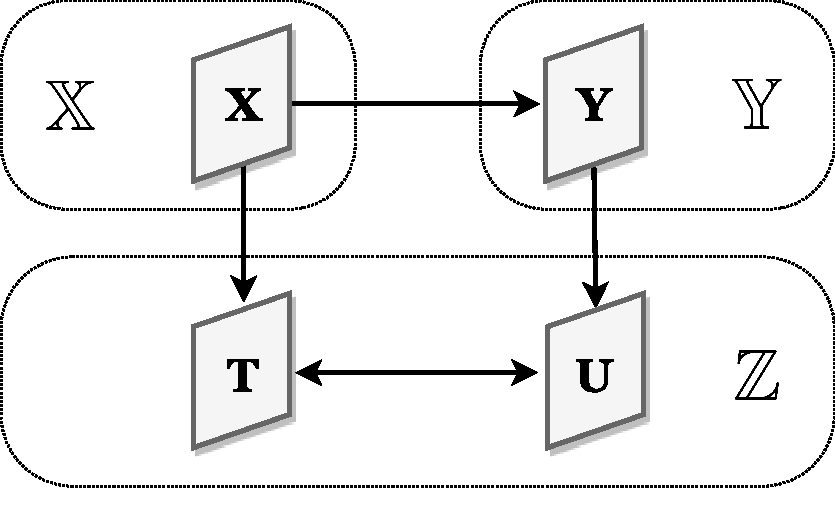
\includegraphics[width=0.4\linewidth]{figs/PLSscheme.pdf}
	\caption{Схема алгоритма PLS}
	\label{fig::PLSscheme}
\end{figure}

Псевдокод метода регрессии PLS приведен в алгоритме~\ref{PLSR_pseudo}. Алгоритм итеративно на каждом из $l$ шагов вычисляет по одному столбцу $\bt_k$, $\bu_k$, $\bp_k$, $\bq_k$ матриц $\bT$, $\bU$, $\bP$, $\bQ$ соответственно. Предполагается, что вектора новых признаков $\bt_k$ и $\bu_k$ являются линейными комбинациями столбцов матриц $\bX$ и $\bY$ соответственно.

Теоретическое обоснование алгоритма PLS следует из следующих теорем.
\begin{theorem}
Целью алгоритма является максимизация ковариации между векторами $\bt_k$ и $\bu_k$. Этим достигается наилучшее описание пространств матриц $\bX$ и $\bY$, а также их взаимной связи
\[
	\text{cov} (\bt_k, \bu_k) = \text{corr} (\bt_k, \bu_k) \cdot \sqrt{\text{Var}(\bt_k)} \cdot \sqrt{\text{Var}(\bu_k)}.
\]

\end{theorem}
Во внутреннем цикле алгоритма вычисляются вектора $\bw_k$ и $\bc_k$. Из данных векторов строятся матрицы $\bW$ и $\bC$ соответственно
Вектора $\bw_k$, $\bc_k$ являются собственными векторами матриц $\bX_k^{\T} \bY_k \bY_k^{\T} \bX_k$ и $\bY_k^{\T} \bX_k \bX_k^{\T} \bY_k$ соответственно

\begin{equation*}
    \bw_k \varpropto \bX_k^{\T} \bu_k = \bX_k^{\T} \bY_k \bc_k \varpropto \bX_k^{\T} \bY_k \bY_k^{\T} \bt_k = \bX_k^{\T} \bY_k \bY_k^{\T} \bX_k \bw_k,
\end{equation*}
\begin{equation*}
    \bc_k \varpropto \bY_k^{\T} \bt_k = \bY_k^{\T} \bX_k \bw_k \varpropto \bY_k^{\T} \bX_k \bX_k^{\T} \bu_k = \bY_k^{\T} \bX_k \bX_k^{\T} \bY_k \bc_k.
\end{equation*}
\begin{theorem}
Правила обновления векторов $\bw_k$, $\bc_k$ совпадают с итерацией алгоритма поиска максимального собственного значения~\cite{Mises1929}. В результате выполнения внутреннего цикла вектора $\bw_k$ и $\bc_k$ будут являться собственными векторами матриц $\bX_k^{\T} \bY_k \bY_k^{\T} \bX_k$ и $\bY_k^{\T} \bX_k \bX_k^{\T} \bY_k$, соответствующими максимальным собственным значениям.
\end{theorem}
\begin{theorem}
Обновляя вектора по данным правилам, мы максимизируем ковариацию между векторами $\bt_k$ и $\bu_k$
\begin{align*}
    \max_{\bt_k, \bu_k}  \text{cov} (\bt_k, \bu_k)^2 &= \max_{\substack{\|\bw_k\|=1 \\ \|\bc_k\| = 1}} \text{cov} \left( \bX_k \bw_k, \bY_k \bc_k \right)^2 = \max_{\substack{\|\bw_k\|=1 \\ \|\bc_k\| = 1}} \text{cov} \left(\bc_k^{\T}  \bY_k^{\T} \bX_k \bw_k \right)^2 = \\
    &= \max_{\|\bw_k\| = 1} \text{cov} \left\|\bY_k^{\T} \bX_k \bw_k \right\|^2 = \max_{\|\bw_k\| = 1} \bw_k^{\T} \bX_k^{\T} \bY_k \bY_k^{\T} \bX_k \bw_k = \\
    & = \lambda_{\max} \left( \bX_k^{\T} \bY_k \bY_k^{\T} \bX_k \right).
\end{align*}
\end{theorem}
После завершения внутреннего цикла вычисляются вектора $\bp_k$, $\bq_k$ проецированием столбцов матриц $\bX_k$ и $\bY_k$ на вектора $\bt_k$ и $\bu_k$. Для перехода на следующий шаг необходимо вычесть из матриц $\bX_k$ и $\bY_k$ одноранговые аппроксимации $\bt_k \bp_k^{\T}$ и $\bt_k \bc_k^{\T}$
\begin{equation*}
    \bX_{k + 1} = \bX_{k-1} - \bt_k \bp_k^{\T} = \bX - \sum_k \bt_k \bp_k^{\T},
\end{equation*}
\begin{equation*}
    \bY_{k + 1} = \bY_{k-1} - \bt_k \bc_k^{\T} = \bY - \sum_k \bt_k \bc_k^{\T},
\end{equation*}
где матрицы с нижним индексом $k$ составленны из $k$ первых векторов, соответственно.
Выражения для регрессии матрицы $\bX$ и матрицы $\bY$ на полученные ортогональные вектора $\bt_1, \dots, \bt_k$
\begin{equation*}
    \bX = \sum_k \bt_k \bp_k^{\T} + \bX_{k + 1} = \bT_k \bP_k^{\bT} + \bX_{k + 1},
\end{equation*}
\begin{equation*}
    \bY = \sum_k \bt_k \bc_k^{\T} + \bY_{k + 1} = \bT_k \bC_k^{\T} + \bY_{k + 1}.
\end{equation*}

Для перехода из пространства $\bX$ в пространство $\bT$ применяется линейное преобразование
\[
	\bT = \bX \bW (\bP^{\T} \bW)^{-1}.
\]

Для нахождения коэффициентов регрессии $\bB$ преобразуем полученное за $l$ шагов алгоритма выражение для регрессии матрицы $\bY$ в предположении, что $\bY_{l + 1}$ является матрицей невязки, 
\begin{equation*}
    \bY = \bT \bC^{\T} + \bY_{l + 1} = \bX \bW (\bP^{\T} \bW)^{-1} \bC^{\T} + \bY_{l + 1} = \bX \bB + \bY_{l + 1}.
\end{equation*}
Таким образом, 
\begin{equation*}
    \bB = \bW (\bP^{\T} \bW)^{-1} \bC^{\T}.
\end{equation*}

\begin{center}
\begin{algorithm}[h]
\caption{Алгоритм PLSR}
    \label{PLSR_pseudo}
\begin{algorithmic}[1]
\REQUIRE $\bX, \bY, l$;
\ENSURE $\bT, \bU, \bP, \bQ$;
\STATE нормировать матрицы $\bX$ и $\bY$
\STATE инициализировать $\bu_1$ (первый столбец матрицы $\bY$)
\STATE $\bX_1 = \bX; \bY_1 = \bY$
\FOR{$k=1,\dots, l$}
  \REPEAT
  \vspace{0.1cm}
    \STATE $\bw_k := \bX_k^{\T} \bu_k / (\bu_k^{\T} \bu_k); \quad \bw_k: = \frac{\bw_k}{\| \bw_k \|}$
    \vspace{0.1cm}
    \STATE $\mathbf{t_k} := \bX_k \bw_k$
    \vspace{0.1cm}
    \STATE $\bc_k := \bY_k^{\T} \bt_k / (\bt_k^{\T} \bt_k)$
    \vspace{0.1cm}
    \STATE $\bu_k := \bY_k \bc_k/ (\bc_k^{\T} \bc_k)$
  \UNTIL{$\bt_k$ не стабилизируется}
  \vspace{0.1cm}
  \STATE $\bp_k:= \bX_k^{\T}\bt_k/(\bt_k^{\T}\bt_k),\ \bq_k := \bY_k^{\T}\bu_k/(\bu_k^{\T}\bu_k)$
  \vspace{0.2cm}
  \STATE $\bX_{k+1} := \bX_k - \bt_k \cdot \left(\frac{\bX_k^{\T} \bt_k}{\bt_k^{\T} \bt_k}\right)^{\T}$
  \vspace{0.2cm}
  \STATE $\bY_{k + 1} := \bY_k - \bt_k \cdot \left(\frac{\bY_k^{\T} \bt_k}{\bt_k^{\T} \bt_k}\right)^{\T}$ 
\ENDFOR
\end{algorithmic}
\end{algorithm}
\end{center}

%%%%%%%%%%%%%%%%%%%%%%%%%%%%%%%%%%%%%%%%%%%%%%%%%%%%%%%%%%%%%%%%%%%%%%%%%%%%%%
\newpage
\section{Модификация метода частных наименьших квадратов (cnlPLS)}
%%%%%%%%%%%%%%%%%%%%%%%%%%%%%%%%%%%%%%%%%%%%%%%%%%%%%%%%%%%%%%%%%%%%%%%%%%%%%%
Предлагается провести модификацию алгоритма PLS: совершить криволинейное и нелинейное преобразования пространства целевой переменной  и независимой переменной для учета мультиколлинеарности между значениями сигнала в различные моменты времени. Схема модифицированного алгоритма представлена на рис.~\ref{scheme_cnlPLS}. 
После применения к исходным матрицам $\bX$ и $\bY$ нелинейных преобразований $F_x$ и $F_y$ соответственно используется линейный алгоритм метода частных наименьших квадратов.

%FIGURE 2

\tikzstyle{sensor_x}=[draw, line width=0.3mm, fill=blue!0, text centered, minimum height=5em, text width=3em]
\tikzstyle{sensor_t}=[draw, line width=0.3mm, fill=blue!0, text centered, minimum height=5em, text width=2em]
\tikzstyle{sensor_p}=[draw, line width=0.3mm, fill=blue!0, text centered, minimum height=2em, text width=3em]
\tikzstyle{sensor_y}=[draw, line width=0.3mm, fill=blue!0, text centered, minimum height=5em, text width=2.5em]
\tikzstyle{sensor_q}=[draw, line width=0.3mm, fill=blue!0, text centered, minimum height=2em, text width=2.5em]

\hspace{1cm}
\begin{figure}[H]
\centering
\begin{tikzpicture}
    \node (x) [sensor_x]  {$\tilde \bX$};
    \node[sensor_x, left of = x, node distance=7.5em] (x_init) {$\bX$};
    % \arrow{x_init,x}{h_y(\breve \bY)}
    \node[right of = x_init, node distance=3.7em] (x_trans) {$\overset{F_x(\bX, \bv_x)}{\longrightarrow}$};
    \node[right of = x, node distance=3em] (x_equal) {=};
    \node[sensor_t, right of = x_equal, node distance=2.5em] (t) {$\bT$};
    \node[right of = t, node distance=2.5em] (x_times) {$\times$};
    \node[sensor_p, right of = x_times, node distance=2.8em] (p) {$\bP^{\T}$};
    \node[right of = p, node distance=2.8em] (x_sum) {+};
    \node[sensor_x, right of = x_sum, node distance=2.8em] (e) {$\bE$};
    % \node[below of = x, node distance=3.5em] (x_size) {\footnotesize{$m\times n$}};
    % \node[below of = t, node distance=3.5em] (t_size) {\footnotesize{$m\times l$}};
    % \node[below of = p, node distance=2.3em] (p_size) {\footnotesize{$l\times n$}};
    % \node[below of = e, node distance=3.5em] (e_size) {\footnotesize{$m\times n$}};

    \node[below of = x_init, node distance=7em] (y_init) [sensor_y]  {$\bY$};
    \node[below of = x_trans, node distance=7em] (y_trans) {$\overset{F_y(\bY, \bv_y)}{\longrightarrow}$};
    \node[below of = x, node distance=7em] (y) [sensor_y]  {$\tilde \bY$};
    \node[below of = x_equal, node distance=7em] (y_equal) {=};
    \node[sensor_t, below of = t, node distance=7em] (u) {$\bU$};
    \node[below of = x_times, node distance=7em] (y_times) {$\times$};
    \node[sensor_q, below of = p, node distance=7em] (q) {$\bQ^{\T}$};
    \node[below of = x_sum, node distance=7em] (y_sum) {+};
    \node[sensor_y, below of = e, node distance=7em] (f) {$\bF$};
\end{tikzpicture}
\caption{Размерности векторов в алгоритме cnlPLS}
\label{scheme_cnlPLS}
\end{figure}


% FIGURE 2 OLD

% \tikzstyle{sensor_x}=[draw, fill=blue!0, text width=4em, 
%     text centered, minimum height=5em]
% \tikzstyle{sensor_y}=[draw, fill=blue!0, text width=2.7em, 
%     text centered, minimum height=5em]
% \begin{figure}[H]
% \centering
% {\footnotesize
% \def\blockdist{2.3}
% \def\edgedist{2.5}
% \vspace{1cm}
% \hspace{1cm}
% \begin{tikzpicture}

%     \node (x) [sensor_x]  {$\bX$};
%     \path (x.south)+(0,-2) node (tilde_x) [sensor_x] {$\tilde \bX$};
%     \path (x.east)+(4,0) node (y) [sensor_y] {$\bY$};
%     \path (y.south)+(0,-2) node (tilde_y) [sensor_y] {$\tilde \bY$};
%     \path (tilde_x.south)+(0,-0.8) node (x_form) {$\tilde \bX = \bT \bP^{T} + \bE$};
%     \path (tilde_y.south)+(0.4,-0.8) node (y_form) {$\tilde \bY = \bU \bQ^{\T} + \bF$};
%     \path (tilde_x.south)+(2.5,-1.3) node (u_form) {$\bU \approx \bT \bD$};


%     \path [draw, ->] (x.south) -- node [right] {$F_x(\bX, \bv_x)$} 
%         (tilde_x.north);
%     \path [draw, ->] (y.south) -- node [right] {$F_y(\bY, \bv_y)$} 
%         (tilde_y.north);
%     %tilde X
%     \path [draw, -] +(1,-2) -- node [right] {$\bt$}
%       +(1,-3.7);
%     \path [draw, -] +(0.8,-3.9) -- node [below] {$\bp$}
%       +(-0.8,-3.9); 
%     %tilde Y
%     \path [draw, -] +(4.05,-2) -- node [left] {$\bu$}
%       +(4.05,-3.7);
%     \path [draw, -] +(4.2,-3.9) -- node [below] {$\bq$}
%       +(5.4,-3.9);

%     \path [draw, ->] +(0.79,-3.77) -- node [above] {$\bw$}
%       +(2.31,-4.8);
%     \path [draw, ->] +(4.21,-3.77) -- node [above] {$\bc$}
%       +(1.9,-4.8);
% \end{tikzpicture}
% }
% \caption{Схема модифицированного метода частных наименьших квадратов}
% \label{scheme_cnlPLS}
% \end{figure}

%%%%%%%%%%%%%%%%%%%%%%%%%%%%%%%%%%%%%%%%%%%%%%%%%%%%%%%%%%%%%%%%%%%%%%%%%%%%%%
\subsection{Нелинейные преобразования}
%%%%%%%%%%%%%%%%%%%%%%%%%%%%%%%%%%%%%%%%%%%%%%%%%%%%%%%%%%%%%%%%%%%%%%%%%%%%%%

    Рассматриваются нелинейное параметрическое преобразование пространства зависимой переменной $\bY$
    и независимой переменной $\bX$ (примеры преобразований представлены в табл.~\ref{table_functions}). Преобразование и вектор параметров, относящиеся к зависимой переменной и независимой переменной, обозначим соответственно $F_y(\bY, \bv_y)$ и $F_x(\bX, \bv_y)$ и введем переменные для преобразованных пространств
    \begin{equation}
    \label{transf}
        \tilde \bY = F_y (\bY, \bv_y),\quad \tilde \bX = F_x(\bX, \bv_x).
    \end{equation}  

    % $\begin{diagram}
    % \node{\bY}
    % \arrow{e,t}{g_y(\bY, \bv_y)}
    % \node{\breve \bY}
    % \arrow{e,t}{h_y(\breve \bY)}
    % \node{\tilde \bY}
    % \end{diagram}$
 
% \begin{table}
% \centering
% \begin{tabular}{l|l|l|l|}
% \cline{2-4}
%   & \textbf{Функция}                                 & \textbf{Параметры} & \textbf{Обратная}                                             \\ \cline{2-4} 
% 1 & $g(x) = \sign(x)\exp(a)(\exp(b|x|) - 1$          & $a, b > 0$         & $g^{-1}(y) = \sign(y) \exp(-b)\log(|y| \exp(-a) + 1)$         \\ \cline{2-4} 
% 2 & $g(x) = \sign(x)\exp(a)(\exp(b\ln(1+ \,|x|) - 1$ & $a, b > 0$         & $g^{-1}(y) = \sign(y)\exp( \exp(-b)\log(|y| \exp(-a) + 1)-1)$ \\ \cline{2-4} 
% 3 & $g(x) = \sign(x)\exp(a)(\exp(b|x|^{1/2}) - 1$    & $a, b > 0$         & $g^{-1}(y) = \sign(y) (\exp(-b)\log(|y| \exp(-a) + 1))^2$     \\ \cline{2-4} 
% 4 & $g(x) = \sign(x)\exp(a)(\exp(b|x|^{1/3}) - 1$    & $a, b > 0$         & $g^{-1}(y) = \sign(y) (\exp(-b)\log(|y| \exp(-a) + 1))^3$     \\ \cline{2-4} 
% 5 & $g(x) = \sign(x)\exp(a)(\exp(b|x|^{1/4}) - 1$    & $a, b > 0$         & $g^{-1}(y) = \sign(y) (\exp(-b)\log(|y| \exp(-a) + 1))^4$     \\ \cline{2-4} 
% 6 & $g(x) = \sign(x)\exp(a)(\exp(b|x|^{2}) - 1$      & $a, b > 0$         & $g^{-1}(y) = \sign(y) (\exp(-b)\log(|y| \exp(-a) + 1))^{1/2}$ \\ \cline{2-4} 
% \end{tabular}
% \caption{Криволинейные преобразования}
% \label{table_functions}
% \end{table}

Функции для криволинейных преобразований удовлетворяют следующим условиям:
\begin{itemize}
    \item $F: \mathbb{R} \to \mathbb{R}$,
    \item $F(0) = 0$,
    \item $F$ дифференцируется по параметрам $\bv_y$,
    \item существует $F^{-1}$.
\end{itemize}

\begin{table}[h]
\centering
\begin{tabular}{|l|l|l|}
\hline
\textbf{№} & \textbf{Функция}                                  & \textbf{Параметры} \\ \hline
1          & $F(x) = \sign(x)\exp(a)(\exp(b|x|) - 1)$          & $a, b > 0$         \\ \hline
2          & $F(x) = \sign(x)\exp(a)(\exp(b\ln(1+ \,|x|) - 1)$ & $a, b > 0$         \\ \hline
3          & $F(x) = \sign(x)\exp(a)(\exp(b|x|^{1/2}) - 1)$    & $a, b > 0$         \\ \hline
4          & $F(x) = \sign(x)\exp(a)(\exp(b|x|^{1/3}) - 1)$    & $a, b > 0$         \\ \hline
5          & $F(x) = \sign(x)\exp(a)(\exp(b|x|^{1/4}) - 1)$    & $a, b > 0$         \\ \hline
6          & $F(x) = \sign(x)\exp(a)(\exp(b|x|^{2}) - 1)$      & $a, b > 0$         \\ \hline
\end{tabular}
\caption{Нелинейные преобразования}
\label{table_functions}
\end{table}



Для обучения параметров $\bv_y$ используется градиентный метод. 
Предлагается подход для обновления весов $\bv_y$, основаный на линеаризации функции преобразования. Разложим (\ref{transf}) в ряд Тейлора до второго порядка: 
$$
    \bu \approx \bu_{0} + \frac{\partial \bu}{\partial \bv_y} \Delta \bv_y.
$$
    
Для вычисления $\Delta \bv_y$ предложены следующие шаги. Рассматривается разница $\bu - \bu_{0} = \frac {\partial \bu}{\partial \bv_y} \Delta \bv_y$. Определется рассогласование
$$
    \bu - \bu_{0} \approx \frac {\partial \bu}{\partial \bv_y} \Delta \bv_y = \bJ_u \Delta \bv_y,
$$
где матрица $\bJ_u$ состоит из частных производных $\left\{\frac {\partial \bu}{\partial \bv_y} \right\}$, вычисленных при известном значении переменной $\bu$: 
\[
    \bJ_u = \frac {\partial \bu}{\partial \bv_y} 
    = \frac {\partial }{\partial \bv_y} (\tilde \bY \bc)
    = \frac1{(\bt^{\T}\bt)} \frac {\partial }{\partial \bv_y} \left(\tilde \bY \tilde \bY^{\T}\bt \right) 
    = \frac{1}{(\bt^{\T}\bt)} \left( \frac {\partial \tilde \bY }{\partial \bv_y}  \cdot \tilde \bY^{\T}  + \tilde \bY \cdot \frac {\partial \tilde \bY^{\T}  }{\partial \bv_y}  \right) \bt.
\]

Правило обновления для вектора $\Delta \bv$ является решением задачи регрессии рассогласования
\begin{equation}
\label{delta_v}
\Delta \bv_y  = (\bJ_u^{\T} \bJ_u)^{-1} \bJ_u^{\T} (\bu - \bu_0).
\end{equation}


Аналогично преобразованию зависимой переменной сводим задачу обновления вектора параметров $\bv_x$ к задаче линейной регрессии:

\begin{align*}
    \bt - \bt_0 \approx \frac {\partial \bt}{\partial \bv_x} \Delta \bv_x = \bJ_t \Delta \bv_x \\
    \Delta \bv_x  = (\bJ_t^{\T} \bJ_t)^{-1} \bJ_t^{\T} (\bt - \bt_0).
\end{align*}

%%%%%%%%%%%%%%%%%%%%%%%%%%%%%%%%%%%%%%%%%%%%%%%%%%%%%%%%%%%%%%%%%%%%%%%%%%%%%%
\subsection{Преобразование независимой переменной}
%%%%%%%%%%%%%%%%%%%%%%%%%%%%%%%%%%%%%%%%%%%%%%%%%%%%%%%%%%%%%%%%%%%%%%%%%%%%%%
    % Аналогично преобразованию целевой переменной $\bY$, совершается преобразование зависимой переменной $\bX$ для учета мультиколлинеарности в признаковом пространстве. 

    % Рассмотрим преобразования $\bX$
    % \begin{itemize} 
    % \item криволинейное с вектором параметров $\bv$ (табл.~\ref{table_functions})
    % \begin{equation}
    % \label{transF_y}
    %     \breve \bX = g_x (\bX, \bv_x),
    % \end{equation}
    % \item нелинейное непараметрическое преобразование
    % \begin{equation*}
    %     \hat \bX = h_x (\bX),
    % \end{equation*}
    % \item суперпозиция преобразований 
    % \begin{equation*}
    %     \tilde \bX = h_x (\breve \bX) = h_x( g_x( \bX, \bv_x)) = F_x(\bX, \bv_x).
    % \end{equation*}
    % \end{itemize}


%%%%%%%%%%%%%%%%%%%%%%%%%%%%%%%%%%%%%%%%%%%%%%%%%%%%%%%%%%%%%%%%%%%%%%%%%%%%%%
\subsection{Алгоритм cnlPLSR}
%%%%%%%%%%%%%%%%%%%%%%%%%%%%%%%%%%%%%%%%%%%%%%%%%%%%%%%%%%%%%%%%%%%%%%%%%%%%%%
В данном разделе представлен модифицированный метод PLSR, содержащий шаги преобразования целевой переменной. Аналогично методу PLSR (алгоритм~\ref{PLSR_pseudo}), алгоритм \ref{cnlPLSR_pseudo} начинается с инициализации вектора $\bu$, а обновления весов преобразования считается с помощью рассогласования $\be$ для вектора $\bu$, вычисленного в цикле и на предыдущей итерации.
\vspace{-0.5cm}

\begin{center}
\begin{algorithm}[h]
\caption{Алгоритм cnlPLSR с преобразованием пространства объектов 2}
    \label{cnlPLSR_pseudo_x}
\begin{algorithmic}[1]
\REQUIRE $\bX, \bY, l$;
\ENSURE $\bT, \bU, \bP, \bQ, \bv_x, \bv_y$;
\STATE инициализировать $\bv_x$ и $\bv_y$
\STATE $\bT := \bU := \bP := \bQ := \emptyset$
\FOR{$k=1,\dots, l$}
\STATE инициализировать $\bt$ (первый столбец матрицы $\bX$)
\STATE инициализировать $\bu$ (первый столбец матрицы $\bY$)
  \REPEAT
  \STATE $\bt_0 := \bt$, $\bu_0 = \bu$
  \vspace{0.1cm}
    \STATE $\tilde \bX := F_x(\bX, \bv_x); \quad \tilde \bY = F_y(\bY, \bv_y)$
    \vspace{0.1cm}
    \STATE $\bw := \tilde \bX^{\T} \bu / (\bu^{\T} \bu); \quad \bw: = \frac{\bw}{\|\bw \|}$
    \STATE $\bt := \tilde \bX \bw$
    \vspace{0.1cm}
    \STATE $\Delta \bv_x = (\bJ_t^{\T} \bJ_t)^{-1} \bJ_t^{\T} (\bt - \bt_0)$, где $\bJ_t := \frac{\partial \bt}{\partial \bv_x}$
    \vspace{0.1cm}
    \STATE $\bv_x := \bv_x + \Delta \bv_x$
    \vspace{0.1cm}
    \STATE $\bc := \tilde \bY^{\T} \bt / (\bt^{\T} \bt); \quad \bc: = \frac{\bc}{\| \bc \|}$ 
    \STATE $\bu := \tilde \bY \bc$
    \vspace{0.1cm}
    \STATE $\Delta \bv_y = (\bJ_u^{\T} \bJ_u)^{-1} \bJ_u^{\T} (\bu - \bu_0)$, где $\bJ_u := \frac{\partial \bu}{\partial \bv_y}$
    \vspace{0.1cm}
    \STATE $\bv_y := \bv_y + \Delta \bv_y$
  \UNTIL{$\bt$ не стабилизируется}
   \vspace{0.1cm}
 \STATE $\bT := \text{concat}[\bT; \bt]$; $\bU := \text{concat}[\bU; \bu]$
 \vspace{0.1cm}
 \STATE $\bp := \tilde \bX^{\T}\bt/(\bt^{\T}\bt),\ \bq := \tilde \bY^{\T}\bu/(\bu^{\T}\bu)$
 \vspace{0.1cm}
 \STATE $\bP:= \text{concat}[\bP; \bp]$; $\bQ := \text{concat}[\bQ; \bq]$
 \vspace{0.1cm}
 \STATE $\tilde \bX := \tilde  \bX - \bt \bp^{\T}$
 \vspace{0.1cm}
 \STATE $\tilde \bY := \tilde  \bY - \bt\bc^{\T}$ 
 \vspace{0.1cm}
  \STATE $\bX = F_x^{-1}(\tilde \bX, \bv_x)$; $\bY = F_y^{-1}(\tilde \bY, \bv_y)$
\ENDFOR
\end{algorithmic}
\end{algorithm}
\end{center}

%%%%%%%%%%%%%%%%%%%%%%%%%%%%%%%%%%%%%%%%%%%%%%%%%%%%%%%%%%%%%%%%%%%%%%%%%%%%%%
\newpage
\section{Вычислительный эксперимент}
%%%%%%%%%%%%%%%%%%%%%%%%%%%%%%%%%%%%%%%%%%%%%%%%%%%%%%%%%%%%%%%%%%%%%%%%%%%%%%

В случае данных электроэнергии $i$-ая строка  матрицы $\bX$~--– локальная история сигнала ($n$ значений сигнала, начиная с момента $i$), а $i$-ая строка матрицы $\bY$~--– локальный прогноз, то есть $r$ значений сигнала, начиная с момента $n+1$. В случае данных ECoG матрица $\bX$ состоит из пространственно-временного спектрального представления временных рядов напряжения, а матрица $\bY$ содержит информацию о положении руки. Процесс генерации матрицы $\bX$ из значений напряжения описан в (ссылка на Мотренко). 

В рамках вычислительного эксперимента строится прогноз временных рядов. В ходе эксперимента сравниваются методы PLSR, нелинейных автоэнкодеров и cnlPLS. Сравнение проводится на реальных данных объемов потребления электроэнергии в Польше. 

Вычислительный эксперимент, продемонстрированный в этом разделе, основан на данных электроэнергии. Данные состоят из временного ряда польских электрических нагрузок и временных рядов погоды в Варшаве (долгота: 21,25, широта: 52,30, высота над уровнем моря: 94). Временные ряды энергии состоят из почасовых записей (всего 52512 наблюдений), а погодные измерения проводились раз в день и содержат 2188 наблюдений. Многомасштабные временные ряды соответствуют периоду 1999-2004 годов. Результаты, полученные с этим набором данных, являются иллюстрацией предлагаемых методов, поскольку данные содержат многомасштабне временные ряды, имеющие различный характер.

Примеры работы алгоритма приведены на рис.~\ref{fig:forecast}. Метод успешно делает краткосрочный прогноз (до 10 дней). С увеличением горизонта прогнозирования предсказание смещается. 


% Require \usepackage{subfig}

% \begin{figure}[H]
%     \centering
%     \begin{subfigure}[b]{0.3\textwidth}
%         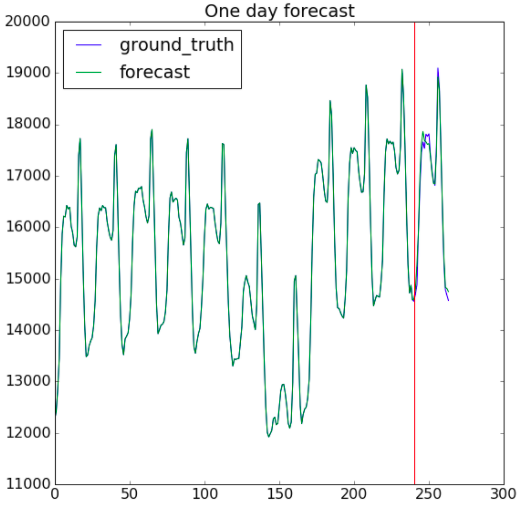
\includegraphics[width=\textwidth]{oneday.png}
%     \end{subfigure}
%     \begin{subfigure}[b]{0.3\textwidth}
%         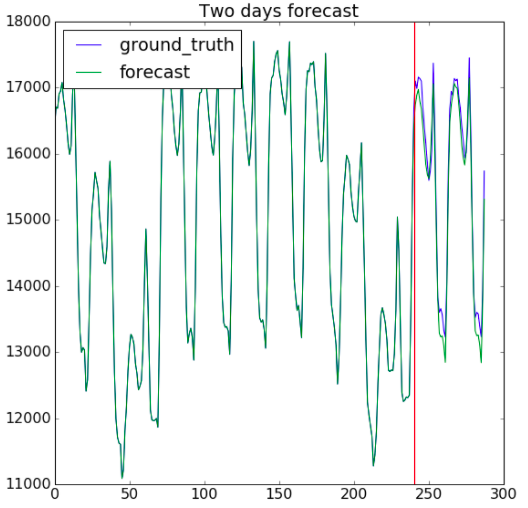
\includegraphics[width=\textwidth]{twodays.png}
%     \end{subfigure}
%     \begin{subfigure}[b]{0.3\textwidth}
%         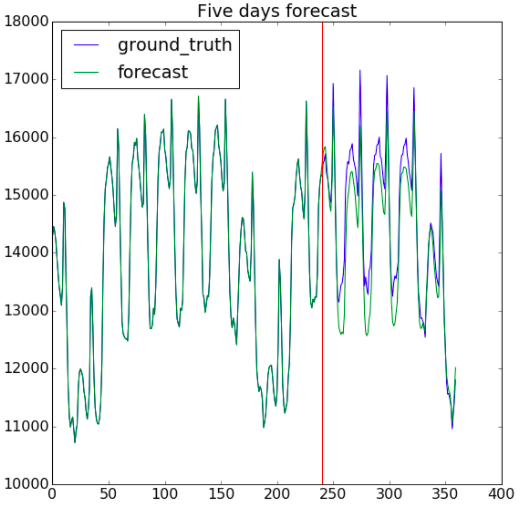
\includegraphics[width=\textwidth]{fivedays.png}
%     \end{subfigure}
%     \begin{subfigure}[b]{0.3\textwidth}
%         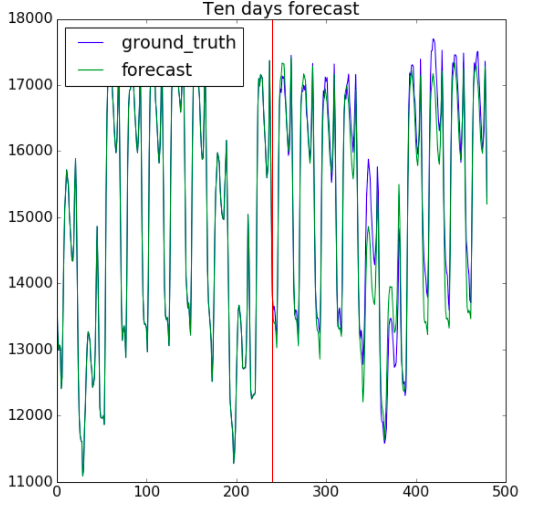
\includegraphics[width=\textwidth]{tendays.png}
%     \end{subfigure}
%     \begin{subfigure}[b]{0.3\textwidth}
%         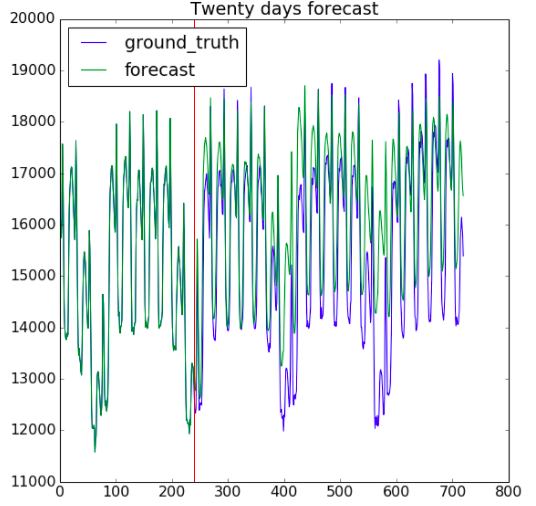
\includegraphics[width=\textwidth]{twentydays.png}
%     \end{subfigure}
%     \begin{subfigure}[b]{0.3\textwidth}
%         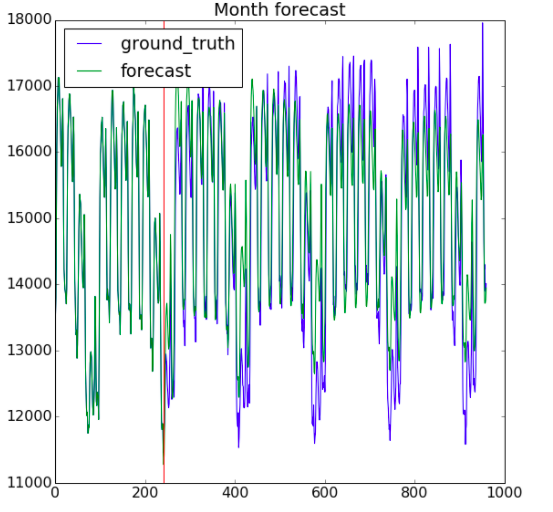
\includegraphics[width=\textwidth]{month.png}
%     \end{subfigure}
%     \caption{Прогнозирование базового алгоритма на 1, 2, 5, 10, 20, 30 дней}
%     \label{fig:forecast}
% \end{figure}

Результаты вычислительного эксперимента для предложенного модифицированного алгоритма cnlPLS представлены на рис.~\ref{fig:animals}. На графиках изображены сглаженные зависимости ошибки MSE от числа компонент в алгоритме для разных функций. Из графиков видно, что для функций $(a)-(e)$ ошибка при увеличении числа компонент падает, затем колеблется, слабо меняясь. Ошибка алгоритма с функцией $(f)$ увеличивается при увеличении числа компонент. Это означает, что преобразование, выполненное в пространстве целевой переменной с помощью функции $(f)$, плохо описывает зависимость. Меньшую ошибку имеют функции, растущие медленнее, а именно $(d)$ и $(e)$. 



% Require \usepackage{subfig}

% \begin{figure}
%     \centering
%     \begin{subfigure}[b]{0.4\textwidth}
%         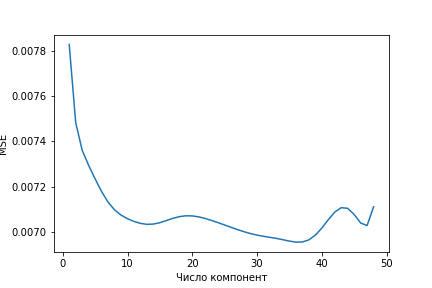
\includegraphics[width=\textwidth]{exp_abs_x.png}
%         \caption{$g(x) = \sign(x) e^a(\exp(b|x|) - 1)$}
%         \label{fig:exp_abs_x}
%     \end{subfigure}
%     ~ %add desired spacing between images, e. g. ~, \quad, \qquad, \hfill etc. 
%       %(or a blank line to force the subfigure onto a new line)
%     \begin{subfigure}[b]{0.4\textwidth}
%         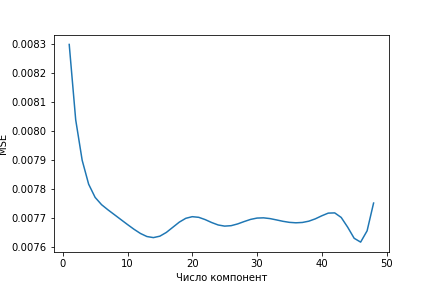
\includegraphics[width=\textwidth]{exp_log_x.png}
%         \caption{$g(x) = \sign(x)e^a(\exp(b\ln(1+ \,|x|) - 1)$}
%         \label{fig:exp_log_x}
%     \end{subfigure}
%     ~ %add desired spacing between images, e. g. ~, \quad, \qquad, \hfill etc. 
%     %(or a blank line to force the subfigure onto a new line)
%     \begin{subfigure}[b]{0.4\textwidth}
%         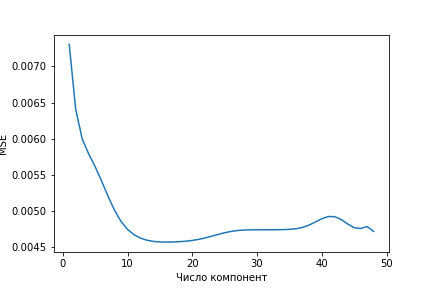
\includegraphics[width=\textwidth]{exp_x_1_2.png}
%         \caption{$g(x) = \sign(x)e^a(\exp(b|x|^{1/2}) - 1)$}
%         \label{fig:exp_x_1_2}
%     \end{subfigure}
%     \begin{subfigure}[b]{0.4\textwidth}
%         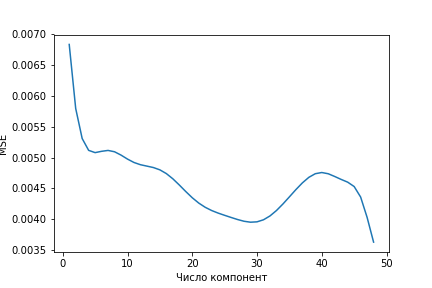
\includegraphics[width=\textwidth]{exp_x_1_3.png}
%         \caption{$g(x) = \sign(x)e^a(\exp(b|x|^{1/3}) - 1)$ }
%         \label{fig:exp_x_1_3}
%     \end{subfigure}
%     ~ %add desired spacing between images, e. g. ~, \quad, \qquad, \hfill etc. 
%       %(or a blank line to force the subfigure onto a new line)
%     \begin{subfigure}[b]{0.4\textwidth}
%         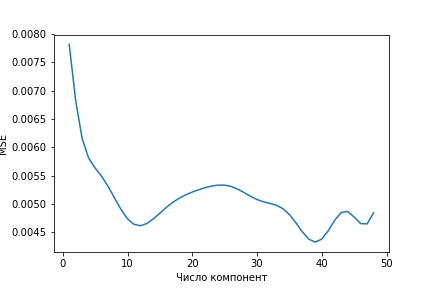
\includegraphics[width=\textwidth]{exp_x_1_4.png}
%         \caption{$g(x) = \sign(x)e^a(\exp(b|x|^{1/4}) - 1)$}
%         \label{fig:exp_x_1_4}
%     \end{subfigure}
%     ~ %add desired spacing between images, e. g. ~, \quad, \qquad, \hfill etc. 
%     %(or a blank line to force the subfigure onto a new line)
%     \begin{subfigure}[b]{0.4\textwidth}
%         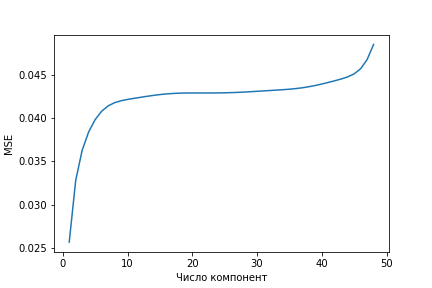
\includegraphics[width=\textwidth]{exp_x_2.png}
%         \caption{$g(x) = \sign(x)e^a(\exp(b|x|^{2}) - 1)$}
%         \label{fig:exp_x_2}
%     \end{subfigure}
%     \caption{Зависимость ошибки от числа компонент в алгоритме cnlPLS для разных функций}\label{fig:animals}
% \end{figure}

В табл.~\ref{results} продемонстрировано увеличение точности прогнозивания при использовании криволинейного преобразования в пространстве зависимой переменной, но увеличение точности в пределах погрешности алгоритма (0.0005-0.0010). Функции с быстрым ростом не позволяют описать зависимость.
\begin{table}[]
\centering
\begin{tabular}{|l|l|l|l|l|}
\hline
\textbf{Алгоритм}                                                                                  & \textbf{N=3}     & \textbf{N=5}     & \textbf{N=10}    & \textbf{N=20}    \\ \hline
PLS                                                                                                & 0,00404          & 0,00337          & \textbf{0,00151} & 0,00135          \\ \hline
\begin{tabular}[c]{@{}l@{}}cnlPLS\\ $g(x) = \sign(x)\exp(a)(\exp(b|x|) - 1)$\end{tabular}          & 0.00529          & 0.00514          & 0.00536          & 0.00506          \\ \hline
\begin{tabular}[c]{@{}l@{}}cnlPLS\\ $g(x) = \sign(x)\exp(a)(\exp(b\ln(1+ \,|x|) - 1)$\end{tabular} & 0.00362          & 0.00386          & 0.00326          & 0.00317          \\ \hline
\begin{tabular}[c]{@{}l@{}}cnlPLS\\ $g(x) = \sign(x)\exp(a)(\exp(b|x|^{1/2}) - 1)$\end{tabular}    & 0.00272          & 0.00236          & 0.00287          & \textbf{0.00128} \\ \hline
\begin{tabular}[c]{@{}l@{}}cnlPLS\\ $g(x) = \sign(x)\exp(a)(\exp(b|x|^{1/3}) - 1)$\end{tabular}    & \textbf{0.00241} & \textbf{0.00233} & 0.00221          & 0.00173          \\ \hline
\begin{tabular}[c]{@{}l@{}}cnlPLS\\ $g(x) = \sign(x)\exp(a)(\exp(b|x|^{1/4}) - 1)$\end{tabular}    & 0.00796          & 0.00768          & 0.00737          & 0.00803          \\ \hline
\begin{tabular}[c]{@{}l@{}}cnlPLS\\ $g(x) = \sign(x)\exp(a)(\exp(b|x|^{2}) - 1)$\end{tabular}      & 0.00816          & 0.00798          & 0.00796          & 0.00775          \\ \hline
\end{tabular}
\caption{Значения ошибки MSE для разных чисел компонент и разных функций}
\label{results}
\end{table}

%%%%%%%%%%%%%%%%%%%%%%%%%%%%%%%%%%%%%%%%%%%%%%%%%%%%%%%%%%%%%%%%%%%%%%%%%%%%%%
\section{Заключение}
В данной работе предложен новый подход к обнаружению зависимостей в пространстве зависимой переменной задачи прогнозирования временных рядов. Сравнивались результаты прогнозирования временных рядов, полученных с помощью метода частных наименьших квадратов и предложенной модификации. Проведен вычислительный эксперимент на реальных данных потребления электроэнергии в Варшаве. Построенная прогностическая модель показала высокое качество предсказания электрической нагрузки. 
%%%%%%%%%%%%%%%%%%%%%%%%%%%%%%%%%%%%%%%%%%%%%%%%%%%%%%%%%%%%%%%%%%%%%%%%%%%%%%
%\section*{СПИСОК ЛИТЕРАТУРЫ}

\newpage
\nocite{*}

\bibliographystyle{unsrt}
\begin{thebibliography}{10}
\def\selectlanguageifdefined#1{
\expandafter\ifx\csname date#1\endcsname\relax
\else\selectlanguage{#1}\fi}

\bibitem{thrun2012}
\BibAuthor{Thrun, Sebastian and Pratt, Lorien}
{Learning to learn}~//
Springer Science \& Business Media, 2012.

\bibitem{Chong2005} %1
%\selectlanguageifdefined{english}
\BibAuthor{Chong, Il Gyo and Jun, Chi Hyuck}
{Performance of some variable selection methods when multicollinearity is present}~//
Chemometrics and Intelligent Laboratory Systems, 2005.
Vol.~78.
No.~1.
P.~103--112.

\bibitem{Xuefeng2010} %1
%\selectlanguageifdefined{english}
\BibAuthor{Xuefeng, Yan}
{Hybrid artificial neural network based on BP-PLSR and its application in development of soft sensors}~//
Chemometrics and Intelligent Laboratory Systems, 2010.
Vol.~103.
No.~2.
P.~152--159.

\bibitem{Mcavovt1992} %1
%\selectlanguageifdefined{english}
\BibAuthor{Mcavovt, J. and Process, Chemical}
{Title }~//
Journal name, 2005.
Vol.~16.
No.~4.
P.~379--391.

\bibitem{Yan2003} %1
%\selectlanguageifdefined{english}
\BibAuthor{Yan, Xuefeng F. and Chen, Dezhao Z. and Hu, Shangxu X.}
{Chaos-genetic algorithms for optimizing the operating conditions based on RBF-PLS model}~//
Computers and Chemical Engineering, 2003.
Vol.~27.
No.~10.
P.~1393--1404.

\bibitem{Frank1990} %1
%\selectlanguageifdefined{english}
\BibAuthor{Frank, Ildiko E.}
{A nonlinear PLS model}~//
Chemometrics and Intelligent Laboratory Systems, 1990.
Vol.~8.
No.~2.
P.~109--119.

\bibitem{Zhou2007} %1
%\selectlanguageifdefined{english}
\BibAuthor{Zhou, Yan Ping and Jiang, Jian Hui and Lin, Wei Qi and Xu, Lu and Wu, Hai Long and Shen, Guo Li and Yu, Ru Qin}
{Artificial neural network-based transformation for nonlinear partial least-square regression with application to QSAR studies}~//
Talanta, 2007.
Vol.~71.
No.~2.
P.~848--853.


\bibitem{Geladi1988} %1
%\selectlanguageifdefined{english}
\BibAuthor{Chong, Il Gyo and Jun, Chi Hyuck}
{Notes on the history and nature of partial least squares (PLS) modelling}~//
Journal of Chemometrics, 1988.
Vol.~2.
No.~January.
P.~231--246.


\bibitem{Hoskuldsson1988} %1
%\selectlanguageifdefined{english}
\BibAuthor{H{\"{o}}skuldsson, Agnar}
{PLS regression}~//
Chemometrics and Intelligent Laboratory Systems, 1987.
Vol.~2.
No.~August.
P.~581--591.


\bibitem{Bulut2014} %1
%\selectlanguageifdefined{english}
\BibAuthor{Bulut, Elif and Egrioglu, Erol}
{A New Partial Least Square Method Based on Elman Neural Network}~//
Chemometrics and Intelligent Laboratory Systems, 2005.
Vol.~4.
No.~4.
P.~154--158.


\bibitem{Ng2013} %1
%\selectlanguageifdefined{english}
\BibAuthor{Ng, Kee Siong}
{A Simple Explanation of Partial Least Squares}~//
Journal title, 2013.
Vol.~volume.
No.~number.
P.~1--10.


\bibitem{Rosipal2011} %1
%\selectlanguageifdefined{english}
\BibAuthor{Rosipal, Roman}
{Nonlinear partial least squares: An overview}~//
Chemoinformatics and Advanced Machine Learning Perspectives: Complex Computational Methods and Collaborative Techniques, 2011.
Vol.~number.
No.~number.
P.~169--189.


\bibitem{Wold1989} %1
%\selectlanguageifdefined{english}
\BibAuthor{Wold, Svante and Kettaneh-Wold, Nouna and Skagerberg, Bert}
{Nonlinear PLS modeling}~//
Chemometrics and Intelligent Laboratory Systems, 1989.
Vol.~7.
No.~1-2.
P.~53--65.

\bibitem{Rosipal2006} %1
%\selectlanguageifdefined{english}
\BibAuthor{Rosipal, Roman and Kramer, Nicole}
{Overview and Recent Advances in Partial Least Squares}~//
????? C. Saunders et al. (Eds.): SLSFS 2005, LNCS 3940, 2006.
Vol.~?.
No.~?.
P.~34--51.

\bibitem{Lu2004} %1
%\selectlanguageifdefined{english}
\BibAuthor{Lu, Wen-Cong and Chen, Nian-Yi and Li, Guo-Zheng and Yang, Jie}
{Multitask Learning Using Partial Least Squares Method}~//
Proceedings of the Seventh International Conference on Information Fusion; International Society of Information Fusion, 2004.
Vol.~1.
P.~79--84.

\bibitem{Varnek2012} %1
%\selectlanguageifdefined{english}
\BibAuthor{Varnek, Alexandre and Baskin, Igor}
{Machine learning methods for property prediction in chemoinformatics: Quo Vadis?}~//
Journal of Chemical Information and Modeling, 2012.
Vol.~52.
No.~6.
P.~1413--1437.

\bibitem{Lehky2014} %1
%\selectlanguageifdefined{english}
\BibAuthor{Lehky, Sidney R. and Kiani, Roozbeh and Esteky, Hossein and Tanaka, Keiji}
{Dimensionality of object representations in monkey inferotemporal cortex}~//
Neural computation, 2014.
Vol.~1872.
No.~10.
P.~1840--1872.

\bibitem{Abdi2003} %1
%\selectlanguageifdefined{english}
\BibAuthor{Abdi, Herv{\'{e}}}
{Partial Least Squares (PLS) Regression}~//
Encyclopedia for research methods for the social sciences, 2003.
P.~792--795.

\bibitem{Caruana2003} %1
%\selectlanguageifdefined{english}
\BibAuthor{Caruana, Rich and de Sa, Virginia R.}
{Benefitting from the Variables that Variable Selection Discards}~//
Journal of Machine Learning Research, 2003.
Vol.~3.
No.~7-8.
P.~1245--1264.

\bibitem{Mises1929} %1
%\selectlanguageifdefined{english}
\BibAuthor{Mises R. V., Pollaczek‐Geiringer H. }
{Praktische Verfahren der Gleichungsauflösung}~//
ZAMM‐Journal of Applied Mathematics and Mechanics/Zeitschrift für Angewandte Mathematik und Mechanik, 1929.
Vol.~9.
No.~1.
P.~58--77.

\bibitem{Li2016} %1
%\selectlanguageifdefined{english}
\BibAuthor{Li J. et al.}
{Feature selection: A data perspective}~//
arXiv preprint arXiv:1601.07996, 2016.


\end{thebibliography}


\end{document}